
\documentclass[a4paper,11pt]{article}
\usepackage[a4paper, margin=8em]{geometry}

% usa i pacchetti per la scrittura in italiano
\usepackage[french,italian]{babel}
\usepackage[T1]{fontenc}
\usepackage[utf8]{inputenc}
\frenchspacing 

% usa i pacchetti per la formattazione matematica
\usepackage{amsmath, amssymb, amsthm, amsfonts}

% usa altri pacchetti
\usepackage{gensymb}
\usepackage{hyperref}
\usepackage{standalone}

\usepackage{colortbl}

\usepackage{xstring}
\usepackage{karnaugh-map}

% imposta il titolo
\title{Appunti Calcolatori Elettronici}
\author{Luca Seggiani}
\date{2025}

% imposta lo stile
% usa helvetica
\usepackage[scaled]{helvet}
% usa palatino
\usepackage{palatino}
% usa un font monospazio guardabile
\usepackage{lmodern}

\renewcommand{\rmdefault}{ppl}
\renewcommand{\sfdefault}{phv}
\renewcommand{\ttdefault}{lmtt}

% circuiti
\usepackage{circuitikz}
\usetikzlibrary{babel}

% testo cerchiato
\newcommand*\circled[1]{\tikz[baseline=(char.base)]{
\node[shape=circle,draw,inner sep=2pt] (char) {#1};}}

% disponi il titolo
\makeatletter
\renewcommand{\maketitle} {
	\begin{center} 
		\begin{minipage}[t]{.8\textwidth}
			\textsf{\huge\bfseries \@title} 
		\end{minipage}%
		\begin{minipage}[t]{.2\textwidth}
			\raggedleft \vspace{-1.65em}
			\textsf{\small \@author} \vfill
			\textsf{\small \@date}
		\end{minipage}
		\par
	\end{center}

	\thispagestyle{empty}
	\pagestyle{fancy}
}
\makeatother

% disponi teoremi
\usepackage{tcolorbox}
\newtcolorbox[auto counter, number within=section]{theorem}[2][]{%
	colback=blue!10, 
	colframe=blue!40!black, 
	sharp corners=northwest,
	fonttitle=\sffamily\bfseries, 
	title=Teorema~\thetcbcounter: #2, 
	#1
}

% disponi definizioni
\newtcolorbox[auto counter, number within=section]{definition}[2][]{%
	colback=red!10,
	colframe=red!40!black,
	sharp corners=northwest,
	fonttitle=\sffamily\bfseries,
	title=Definizione~\thetcbcounter: #2,
	#1
}

% disponi codice
\usepackage{listings}
\usepackage[table]{xcolor}

\definecolor{codegreen}{rgb}{0,0.6,0}
\definecolor{codegray}{rgb}{0.5,0.5,0.5}
\definecolor{codepurple}{rgb}{0.58,0,0.82}
\definecolor{backcolour}{rgb}{0.95,0.95,0.92}

\lstdefinestyle{codestyle}{
	backgroundcolor=\color{black!5}, 
	commentstyle=\color{codegreen},
	keywordstyle=\bfseries\color{magenta},
	numberstyle=\sffamily\tiny\color{black!60},
	stringstyle=\color{green!50!black},
	basicstyle=\ttfamily\footnotesize,
	breakatwhitespace=false,         
	breaklines=true,                 
	captionpos=b,                    
	keepspaces=true,                 
	numbers=left,                    
	numbersep=5pt,                  
	showspaces=false,                
	showstringspaces=false,
	showtabs=false,                  
	tabsize=2
}

\lstdefinestyle{shellstyle}{
	backgroundcolor=\color{black!5}, 
	basicstyle=\ttfamily\footnotesize\color{black}, 
	commentstyle=\color{black}, 
	keywordstyle=\color{black},
	numberstyle=\color{black!5},
	stringstyle=\color{black}, 
	showspaces=false,
	showstringspaces=false, 
	showtabs=false, 
	tabsize=2, 
	numbers=none, 
	breaklines=true
}


\lstdefinelanguage{assembler}{ 
	keywords={AAA, AAD, AAM, AAS, ADC, ADCB, ADCW, ADCL, ADD, ADDB, ADDW, ADDL, AND, ANDB, ANDW, ANDL,
		ARPL, BOUND, BSF, BSFL, BSFW, BSR, BSRL, BSRW, BSWAP, BT, BTC, BTCB, BTCW, BTCL, BTR, 
		BTRB, BTRW, BTRL, BTS, BTSB, BTSW, BTSL, CALL, CBW, CDQ, CLC, CLD, CLI, CLTS, CMC, CMP,
		CMPB, CMPW, CMPL, CMPS, CMPSB, CMPSD, CMPSW, CMPXCHG, CMPXCHGB, CMPXCHGW, CMPXCHGL,
		CMPXCHG8B, CPUID, CWDE, DAA, DAS, DEC, DECB, DECW, DECL, DIV, DIVB, DIVW, DIVL, ENTER,
		HLT, IDIV, IDIVB, IDIVW, IDIVL, IMUL, IMULB, IMULW, IMULL, IN, INB, INW, INL, INC, INCB,
		INCW, INCL, INS, INSB, INSD, INSW, INT, INT3, INTO, INVD, INVLPG, IRET, IRETD, JA, JAE,
		JB, JBE, JC, JCXZ, JE, JECXZ, JG, JGE, JL, JLE, JMP, JNA, JNAE, JNB, JNBE, JNC, JNE, JNG,
		JNGE, JNL, JNLE, JNO, JNP, JNS, JNZ, JO, JP, JPE, JPO, JS, JZ, LAHF, LAR, LCALL, LDS,
		LEA, LEAVE, LES, LFS, LGDT, LGS, LIDT, LMSW, LOCK, LODSB, LODSD, LODSW, LOOP, LOOPE,
		LOOPNE, LSL, LSS, LTR, MOV, MOVB, MOVW, MOVL, MOVSB, MOVSD, MOVSW, MOVSX, MOVSXB,
		MOVSXW, MOVSXL, MOVZX, MOVZXB, MOVZXW, MOVZXL, MUL, MULB, MULW, MULL, NEG, NEGB, NEGW,
		NEGL, NOP, NOT, NOTB, NOTW, NOTL, OR, ORB, ORW, ORL, OUT, OUTB, OUTW, OUTL, OUTSB, OUTSD,
		OUTSW, POP, POPL, POPW, POPB, POPA, POPAD, POPF, POPFD, PUSH, PUSHL, PUSHW, PUSHB, PUSHA, 
		PUSHAD, PUSHF, PUSHFD, RCL, RCLB, RCLW, MOVSL, MOVSB, MOVSW, STOSL, STOSB, STOSW, LODSB, LODSW,
		LODSL, INSB, INSW, INSL, OUTSB, OUTSL, OUTSW
		RCLL, RCR, RCRB, RCRW, RCRL, RDMSR, RDPMC, RDTSC, REP, REPE, REPNE, RET, ROL, ROLB, ROLW,
		ROLL, ROR, RORB, RORW, RORL, SAHF, SAL, SALB, SALW, SALL, SAR, SARB, SARW, SARL, SBB,
		SBBB, SBBW, SBBL, SCASB, SCASD, SCASW, SETA, SETAE, SETB, SETBE, SETC, SETE, SETG, SETGE,
		SETL, SETLE, SETNA, SETNAE, SETNB, SETNBE, SETNC, SETNE, SETNG, SETNGE, SETNL, SETNLE,
		SETNO, SETNP, SETNS, SETNZ, SETO, SETP, SETPE, SETPO, SETS, SETZ, SGDT, SHL, SHLB, SHLW,
		SHLL, SHLD, SHR, SHRB, SHRW, SHRL, SHRD, SIDT, SLDT, SMSW, STC, STD, STI, STOSB, STOSD,
		STOSW, STR, SUB, SUBB, SUBW, SUBL, TEST, TESTB, TESTW, TESTL, VERR, VERW, WAIT, WBINVD,
	XADD, XADDB, XADDW, XADDL, XCHG, XCHGB, XCHGW, XCHGL, XLAT, XLATB, XOR, XORB, XORW, XORL},
	keywordstyle=\color{blue}\bfseries,
	ndkeywordstyle=\color{darkgray}\bfseries,
	identifierstyle=\color{black},
	sensitive=false,
	comment=[l]{\#},
	morecomment=[s]{/*}{*/},
	commentstyle=\color{purple}\ttfamily,
	stringstyle=\color{red}\ttfamily,
	morestring=[b]',
	morestring=[b]"
}

\lstset{language=assembler, style=codestyle}

% disponi sezioni
\usepackage{titlesec}

\titleformat{\section}
{\sffamily\Large\bfseries} 
{\thesection}{1em}{} 
\titleformat{\subsection}
{\sffamily\large\bfseries}   
{\thesubsection}{1em}{} 
\titleformat{\subsubsection}
{\sffamily\normalsize\bfseries} 
{\thesubsubsection}{1em}{}

% tikz
\usepackage{tikz}

% float
\usepackage{float}

% grafici
\usepackage{pgfplots}
\pgfplotsset{width=10cm,compat=1.9}

% disponi alberi
\usepackage{forest}

\forestset{
	rectstyle/.style={
		for tree={rectangle,draw,font=\large\sffamily}
	},
	roundstyle/.style={
		for tree={circle,draw,font=\large}
	}
}

% disponi algoritmi
\usepackage{algorithm}
\usepackage{algorithmic}
\makeatletter
\renewcommand{\ALG@name}{Algoritmo}
\makeatother

% disponi numeri di pagina
\usepackage{fancyhdr}
\fancyhf{} 
\fancyfoot[L]{\sffamily{\thepage}}

\makeatletter
\fancyhead[L]{\raisebox{1ex}[0pt][0pt]{\sffamily{\@title \ \@date}}} 
\fancyhead[R]{\raisebox{1ex}[0pt][0pt]{\sffamily{\@author}}}
\makeatother

\begin{document}
% sezione (data)
\section{Lezione del 08-04-25}

% stili pagina
\thispagestyle{empty}
\pagestyle{fancy}

% testo
Concluso il discorso sulla memoria virtuale, ci concentreremo nuovamente sull'hardware, nella prospettiva di approfondire l'interazione fra nucleo e dispositivi di I/O. 

\subsection{Bus PCI}
Il bus \textbf{PCI}, che sta per \textit{Peripheral Component Interconnect}, è uno standard per bus sviluppato da IBM per consentire l'espansione dei loro calcolatori attraverso schede apposite, supportando quindi una cosiddetta \textit{architettura aperta}.

Possiamo quindi immaginare che ogni scheda di espansione sia provvista dei suoi registri, delle sue interruzioni, ecc... che non devono sovrapporsi con quelli di altre schede.
Storicamente, questo rappresentava un problema, in quanto potevano crearsi \textit{conflitti} fra più schede.

Inoltre, un problema era rappresentato dai \textit{driver}, in quanto non esisteva un modo standardizzato per rilevare se una certa scheda era installata o no, e quindi se si poteva usare un certo driver.

I produttori stabilirono quindi una sorta di standard \textit{de facto}, che abbiamo già nominato: l'\textbf{ISA} (\textit{Industry Standard Architecture}).

L'idea fondamentale è che la scheda non può avere registri fissi, ma deve essere programmabile in questo dal calcolatore.
Inoltre, deve esistere una qualche modalità per rilevare le schede correntemente installate nel sistema.

Nei PC moderni sfruttiamo uno standard di derivazione dal vecchio PCI, compatibile con esso, che è il \textit{PCI Express} (e che non studieremo).

\subsubsection{Indirizzamento dei dispositivi}
Secondo lo standard PCI, separiamo il \textbf{bus locale} (quello che abbiamo visto finora) da un eventuale \textbf{albero di bus}, collegati fra di loro dai cosiddetti \textbf{ponti}.
Il \textbf{ponte ospite-PCI}, in particolare, collega il \textbf{bus principale} (il più vicino al bus locale) al bus locale, mentre questo a sua volta viene collegato ad altri bus attraverso \textbf{ponti PCI-PCI}.
Ad esempio, molti calcolatori dell'epoca erano dotati di \textit{bus ISA} collegati con appositi ponti al bus principale, per la gestione di vecchie interfacce ISA.

A ogni bus è associato un numero su 8 bit, col bus principale che si prende il numero 0.

Per indirizzare un dispositivo usiamo invece 16 bit, disposti come:
\begin{table}[H]
	\center 
	\begin{tabular} { c | c c }
		\bfseries Scopo & \bfseries Bit & \bfseries Max \\
		\hline 
		\textit{Bus} & 8 bit & 256 \\
		\textit{Device} & 5 bit & 32\\
		\textit{Function} & 3 bit & 8
	\end{tabular}
\end{table}
dove il numero di bus è lo stesso di prima.

Il numero di dispositivo differisce dal \textit{Device ID}, che vedremo fra poco, e deriva dalla posizione fisica del dispositivo nel bus.

Il numero di funzione, invece, è reso necessario da schede che implementano più funzionalità, quali ad esempio le schede grafiche moderne, che si occupano anche dell'audio.
In ogni caso, la funzione 0 deve essere implementata obbligatoriamente.

Come vediamo dalla tabella, poi, si possono avere direttamente dalle codifiche fino a 256 bus diversi, con 32 dispositivi ciascuno e 8 funzioni per dispositivo.

\subsubsection{Operazioni coi dispositivi}
Veniamo quindi a come funzionano le operazioni più semplici sul Bus PCI.
Ogni operazione sul PCI viene detta \textbf{transazione}, ed ha un \textbf{iniziatore} e un \textbf{obiettivo}, cioè il dispositivo che inizia la transazione e il dispositivo che gli risponde.

L'iniziatore delle richieste che il nostro programma invia all'I/O, notiamo, non sarà più il processore, ma il ponte ospite-PCI.
Inoltre, il bus PCI permette in verità che anche dispositivi esterni al ponte ospite-PCI facciano da iniziatori per transazioni, rendendo possibili meccanismi come il \textbf{DMA} (\textit{Direct Memory Access}). 

Sul bus vero e proprio troviamo quindi:
\begin{itemize}
	\item La linea di \textbf{clock}, che tutte le interfacce vedono, originariamente intorno ai 33 MHz.
		Sul fronte di salita del clock tutte le interfacce (idealmente) campionano i segnali sul bus;
	\item \textbf{FRAME\#}, che "incornicia" la transazione corrente: l'iniziatore lo alza quando la transazione è finita. Al massimo, a handshake avvenuto si possono avere un numero indefinito di cili di trasmissione da 4 byte: il FRAME si alza ad avvenuta trasmissione dell'ultimo fra questi;
	\item \textbf{AD}, la linea \textit{condivisa} di indirizzo o dati, a 32 bit;
	\item \textbf{C/BE\#}, \textit{controllo} e \textit{byte-enable}, codificano il tipo di operazione in fase di indirizzamento e fanno da byte-enable nel trasferimento dati;
	\item \textbf{IRDY\#} e \textbf{TRDY\#}, rispettivamente \textit{Initiator Ready} e \textit{Target Ready}, supportano l'handshake nella fase di scambio dati: l'iniziatore abbassa IRDY quando è pronto a ricevere dati o quando inizia a scriverli, mentre l'obiettivo abbassa TRDY quando inizia a inviare dati o a riceverli;
	\item \textbf{DEVSEL\#}, viene attivato dal dispositivo che riconosce, controllando C/BE e l'indirizzo su AD, una chiamata a sé stesso, quindi dal presunto \textit{obiettivo}; 
	\item \textbf{STOP\#}, viene attivato dall'\textit{obiettivo} per terminare prematuramente una transazione.
\end{itemize}
dove il \# indica \textit{attivi bassi}.

\newpage

Vediamo nel dettaglio due transazioni complete, di lettura e scrittura a 4 byte sequenziali, per capire a pieno la politica di handshake:
\begin{itemize}
	\item \textbf{Lettura:} 
	\begin{center}
		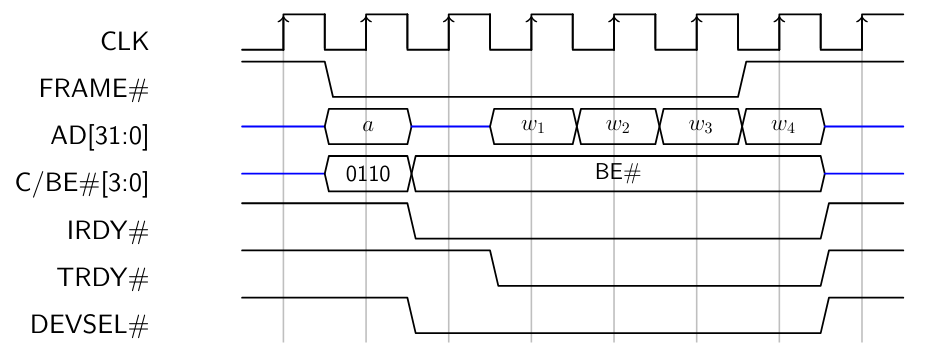
\includegraphics[scale=0.5]{../figures/pci_read.png}
	\end{center}
	Abbiamo che l'iniziatore come prima cosa porta il FRAME in basso e scrive l'indirizzo in AD e la modalità di indirizzamento in C/BE (qui \lstinline|0110|, che significa memoria).
	L'obiettivo risponde abbassando DEVSEL, al cui l'iniziatore risponde abbassando IRDY. 
	Fra l'abbassamento di IRDY e l'inizio della trasmissione (l'abbassamento di TRDY) c'è un ciclo di clock a vuoto, detto \textit{ciclo di turnaround}, che permette all'iniziatore di rilasciare AD e C/BE perchè l'obiettivo possa assumerne il controllo.
	Si trasmettono quindi 16 byte in mandate da 4, con FRAME che torna alto al quarto byte per segnalare la fine dell'operazione, e le linee di handshake (IRDY, TRDY e DEVSEL) tornano alte.

	\item \textbf{Scrittura:} 
	\begin{center}
		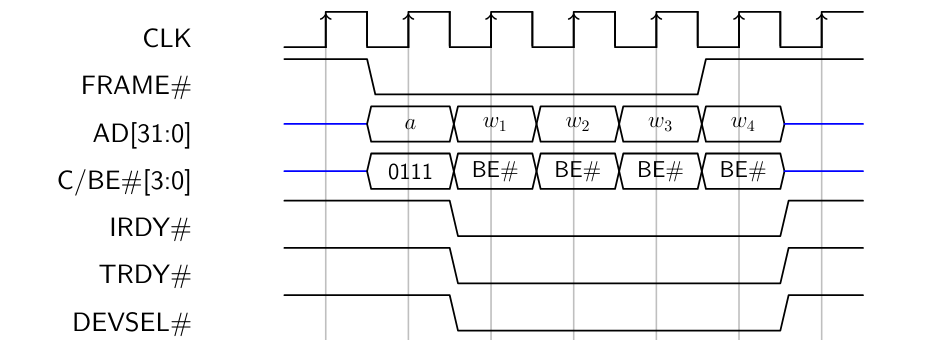
\includegraphics[scale=0.5]{../figures/pci_write.png}
	\end{center}
	Le cose si svolgono in maniera pressoché identica, con la differenza che non si necessita di un ciclo di turnaround in quanto l'iniziatore sarà l'unico a scrivere su AD e C/BE. Inoltre, possiamo immaginare che C/BE venga effettivamente modificato nel corso della scrittura, in quanto magari non vogliamo impattare tutti i byte ad ogni ciclo di scrittura.
\end{itemize}

\subsubsection{Spazio di configurazione}
Per poter lavorare con il bus PCI, poi, introduciamo un nuovo spazio indirizzabile, quello di \textbf{configurazione}.
Avremo quindi che il processore può indirizzare:
\begin{itemize}
	\item \textbf{Memoria};
	\item \textbf{I/O};
	\item \textbf{Configurazione}.
\end{itemize}
Questo spazio è rilevante solo all'avvio del calcolatore (all'esecuzione del BIOS, o come definito originariamente dallo standard, \textit{PCI BIOS}), appunto per effettuare la configurazione delle interfacce PCI installate nel sistema.
Ogni bus PCI trasporta quindi messaggi in uno qualsiasi di questi 3 spazi, e si discrimina lo spazio specifico controllando cosa l'iniziatore mette in C/BE.

Useremo lo spazio di I/O come sempre, ma i segnali del processore viaggeranno attraverso i vari ponti fino all'interfaccia desiderata.
Per quanto riguarda i dispositivi mappati in memoria (si pensi al video), invece, possiamo assumere che all'avvio il ponte ospite-PCI deve solo sapere la dimensione della memoria RAM installata, in modo da rispondere da lì in poi solo agli indirizzi \textit{di memoria} posti al di \textit{sotto} di essa.
Avevamo visto questo meccanismo nella sezione 17.2, vedendo come il bootloader ignora la zona di memoria superiore alla RAM e dedicata al bus PCI.

Notiamo che tutto questo sistema è comunque strutturato per essere trasparente al processore, e quindi invisibile lato software.

\subsubsection{Configurazione dei dispositivi}
Ogni dispositivo sul bus è obbligato a fornire, per ogni funzione e ad una certa locazione predefinita, un numero di registri che formano 64 righe da 32 bit, che devono contenere informazioni di configurazione.
I primi due dati, su 16 bit (quindi una riga), saranno il \textbf{Vendor ID} e il \textbf{Device ID}, seguiti da altri dati che non ci sono immediatamente rilevanti:

\begin{center}
	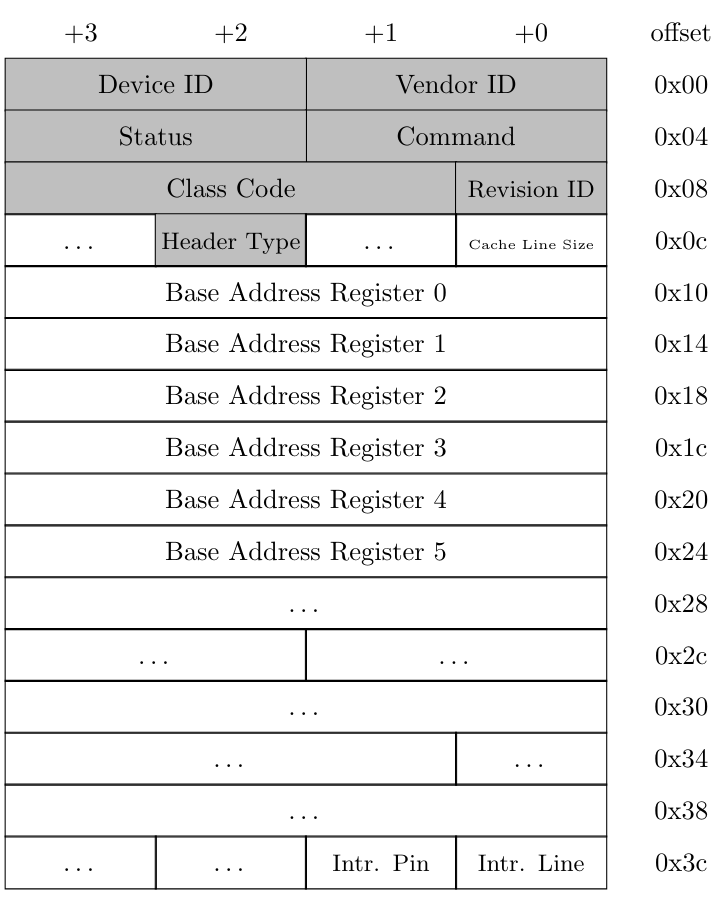
\includegraphics[scale=0.5]{../figures/config_space.png}
\end{center}

Il Vendor ID è determinato da un'autorità centrale (la \textit{PCI-SIG}): ad esempio, il vendor ID della Intel è \lstinline|0x8086|.

Per permettere quindi alla CPU di configurare i dispositivi, cioè accedere ai loro registri di configurazione, il ponte ospite-PCI rende disponibili alla CPU due registri, entrambi su 32 bit:
\begin{itemize}
	\item Il \textbf{CAP}, \textit{Configuration Address Port}, che permette di selezionare una funzione e l'offset della parola a cui si vuole accedere;
	\item Il \textbf{CDP}, \textit{Configuration Data Port}, che permette di accedere alla parola selezionata con \textit{CAP}.
\end{itemize}
Le operazioni effettuate dalla CPU attraverso questi due registri verranno trasformate automaticamente dal ponte ospite-PCI in operazioni di configurazione sui bus PCI.

La posizione di questi registri in memoria è la seguente:
\begin{table}[h!]
	\center
	\begin{tabular} { c | p{7cm} }
		\lstinline|0xcf8| & \textbf{CAP}, \textit{Configuration Address Port} \\
		\lstinline|0xcfc| & \textbf{CDP}, \textit{Configuration Data Port}	
	\end{tabular}
\end{table}

Vediamo quindi cosa deve fare il BIOS per la configurazione dei dispositivi PCI, cioè per collocarne nello spazio di I/O o in memoria eventuali registri o porzioni di memoria, rispettivamente.
Ogni dispositivo ha una \textbf{dimensione naturale} che occupa nello spazio, sia questo di memoria o di I/O.
Fornisce quindi al processore un registro, detto \textbf{BAR} (\textit{Base Address Register}), che è scrivibile solo in parte: la parte meno significativa, infatti, è fissa a 0 e determina la dimensione naturale della regione che questo occuperà.
Per rilevare la dimensione naturale, quindi, basta scrivere tutti 1 sul BAR e controllare quali bit vengono effettivamente modificati.

Il PCI BIOS dovrà quindi, attraverso i registri CAP e CDP, controllare il BAR di tutte le interfacce, determinarne la dimensione naturale e trovare una regione libera nello spazio di I/O o in memoria, a seconda del tipo di dispositivo, dove collocarle.

\subsubsection{Interruzioni PCI}
Per la gestione delle interruzioni, lo standard si ferma al dire che ogni dispositivo deve specificare per ogni funzione quale, di quattro linee di interruzione, tale funzione usa, in un apposito registro di configurazione.
Queste linee sono dette \textbf{INTA}, \textbf{INTB}, \textbf{INTC} e \textbf{INTD}, e lo spazio di configurazione della funzione contiene il dato rispetto a quale linea usa in \textit{Intr. Pin}, con 0 che significa nessuna interruzione, 1 \textit{INTA}, e così via.

\subsubsection{Struttura di un bus PCI}
Per fissare i concetti di quest'ultima sezione, cerchiamo di esporre la struttura del calcolatore emulato su cui abbiamo studiato finora.
Scriviamo quindi un programma che cerchi tutti i dispositivi presenti nella configurazione attuale, sfruttando le funzioni per la gestione dello spazio di configurazione definite in \lstinline|libce.h| (\lstinline|read_conf...()|):
\lstset{style = codestyle, language=c++}
\lstinputlisting{../code/pci/pci.cpp}
e vediamo cosa stampa:
\lstinputlisting{../code/misc/dev.txt}
dove i commenti sono stati aggunti successivamente.

\par\medskip

Vediamo quindi che abbiamo 3 dispositivi, tutti sul bus 0 (bus principale):
\begin{enumerate}
	\item[0:] Il ponte ospite-PCI;
	\item[1:] Un dispositivo che fornisce altri bus, che possiamo individuare nel \textit{southbridge} Intel \textbf{PIIX3} (\textit{PCI IDE ISA Xcelerator}). Questi sono:
		\begin{enumerate}
			\item[0:] Un bus ISA accessibile attraverso il ponte PCI-ISA, che emula le interfacce di tastiera e di timer dell'ISA;
			\item[2:] Un bus ATA accessibile attraverso il ponte PCI-ATA, che permette l'interazione con il disco rigido (hard disk);
			\item[3:] L'interfaccia \textbf{ACPI} (\textit{Advanced Configuration and Power Interface}), non di interesse a questo corso.
		\end{enumerate}
		Il southbridge si interfaccia poi con altri componenti, quali ad esempio l'APIC (ed emula il PIC sul bus ISA).
	\item[2:] La scheda video VGA emulata di \textit{bochs}, un emulatore precedente a QEMU.
\end{enumerate}

\noindent
\begin{minipage}{\textwidth}
La struttura complessiva sarà quindi la seguente:

\begin{center}
	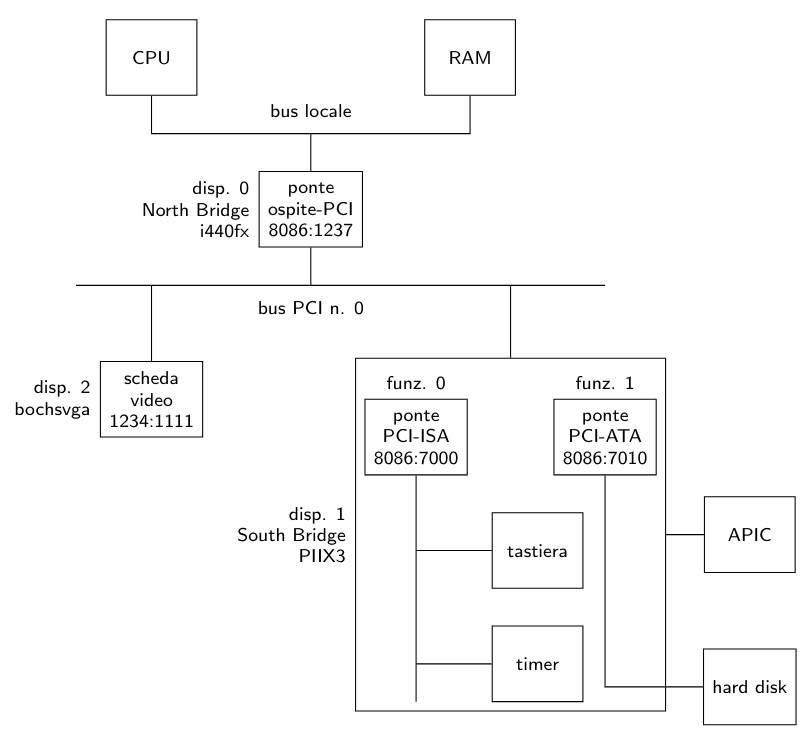
\includegraphics[scale=0.55]{../figures/pci_space.png}
\end{center}

\end{minipage}

\subsection{I/O nel kernel}
La maggior parte delle modifiche allo spazio di I/O apportate introducendo il bus PCI, abbiamo detto, sono effettivamente trasparenti al processore, se non per l'introduzione dei registri CAP e CDP, che devono essere comunque usati una volta sola nel PCI BIOS per la configurazione dei dispositivi.
Possiamo quindi sfruttare la maggior parte delle funzioni definite in \lstinline|libce.h| per l'input/output senza particolari problemi.

Vediamo quindi com'è implementata la gestione dell'I/O da parte del \textit{kernel}.

Avevamo detto che la motivazione principale dietro lo sviluppo del sistema multiprogrammato era che questa permetteva l'interruzione in qualsiasi momento di un \textit{processo} in esecuzione, per permettere al processore di effettuare altre operazioni.
Le interruzioni sollevate da i dispositivi esterni, vediamo, possono essere gli eventi che provocano tale cambio di contesto, e quindi la gestione del segnale in ingresso al sistema.

Ad esempio, un processo potrebbe, con la funzione \lstinline|readconsole()|, specificare un buffer e un numero di caratteri che vuole leggere da tastiera.
A questo punto, il sistema lo metterà in attesa e si occuperà di altro, riempiendo sequenzialmente il buffer via via che i tasti vengono effettivamente premuti (e quindi le relative interruzioni sollevate).
Una volta che il buffer sia riempito dal numero di caratteri richiesti dal processo, potrà quindi rimettere il processo in esecuzione, o nella lista pronti, e proseguire.

Per tenere conto di più processi che possono voler leggere contemporaneamente, poi, ci dotiamo di un semaforo che tenga conto di chi sta usando quella risorsa in un certo momento.
Un problema qui sarà come usare i semafori da lato sistema, e verrà discusso nella prossima lezione.

\end{document}
